\documentclass[journal,onecolumn,11pt,draftclsnofoot]{IEEEtran}
% One-column draft for review. For a two-column workshop submission use
% \documentclass[conference]{IEEEtran} and shorten Sections V-B and VI.

\usepackage[utf8]{inputenc}
\usepackage[T1]{fontenc}
\usepackage{amsmath,amssymb,amsfonts}
\usepackage{graphicx}
\usepackage{booktabs}
\usepackage{multirow}
\usepackage{xcolor}
\usepackage{url}
\usepackage[hidelinks]{hyperref}
\usepackage{cite}

\graphicspath{{../../results/channel/figures/}{figures/}}

\newcommand{\ATS}{\mathrm{ATS}}
\newcommand{\E}{\mathbb{E}}
\newcommand{\Q}{\mathsf{Q}}

\begin{document}

\title{Channel-Aware Semantic Packet Aggregation\\for Token Communication over Bursty and Fading Erasure Channels}

\author{\IEEEauthorblockN{Anonymous authors}\\
\IEEEauthorblockA{Draft for workshop submission. Code and data: \url{https://github.com/poseidon577/sempa-look}}}

\maketitle

\begin{abstract}
Semantic packet aggregation decides which tokens of a message share a packet, so that the message keeps as much of its meaning as possible when packets are lost. Existing methods assume that every packet is erased independently with the same probability. We show that this assumption is costly. On Gilbert--Elliott and correlated Rayleigh-fading channels at the same average loss rate, the state-of-the-art lookahead aggregator keeps as little as 1\% of the attainable gain over random grouping, and even the exhaustively searched i.i.d.-optimal grouping keeps only 32--73\% at six packets per message. Under memory a second degree of freedom appears that i.i.d.\ models hide: the order in which a message's packets are sent. We propose CASA, a channel-aware aggregator that fits a pairwise surrogate of semantic similarity on subsets drawn from the channel's own survival law, reduces expected similarity under the channel's joint loss law to a closed-form quadratic assignment problem, and re-ranks a few local optima exactly. On MS-COCO captions CASA captures 85--92\% of the exhaustive oracle's gain on every channel tested, beats the lookahead aggregator by up to $+0.040$ average token similarity (ATS), and beats the best channel-blind grouping found by exhaustive search. The gains persist on 24- to 60-token WikiHow passages, when partitions are re-scored with two other sentence encoders and with BERTScore, and when the channel law is misspecified or estimated from a short loss trace. \emph{[Mismatch and BERTScore sentences to be finalised with the new runs.]}
\end{abstract}

\begin{IEEEkeywords}
Semantic communication, token communication, packet aggregation, burst erasures, Gilbert--Elliott channel, interleaving.
\end{IEEEkeywords}

%=====================================================================
\section{Introduction}
%=====================================================================

Token communication sends the discrete tokens of a generative model's input or output instead of bits of a waveform~\cite{qiao2025tokcom}. When tokens travel in packets, a lost packet removes several tokens at once, and which tokens share a packet decides how much meaning survives. SemPA-GBeam~\cite{lee2025gbeam} and SemPA-Look~\cite{lee2026look} formalise this as semantic packet aggregation: partition the $K$ tokens of a message into $N$ groups of $M$ tokens to maximise the average token similarity (ATS), the expected sentence-embedding similarity between the received and the original message. SemPA-Look reaches near-exhaustive ATS at linear cost with a residual semantic score and a lookahead search.

Both methods assume that packets are erased independently. Real links are bursty: fading, interference and congestion make consecutive losses far more likely than independent losses at the same average rate. For compressed video it has long been known that distortion depends on burst length, not only on the loss rate~\cite{liang2003burst}. We ask the same question for semantic aggregation and find that the answer changes the problem in two ways. First, the grouping that is optimal under independent losses is far from optimal under memory. Second, the \emph{slot order}, i.e.\ which group rides in which of the message's transmission slots, starts to matter, because slots that are close in time tend to fail together.

Prior work on loss-resilient token and feature transmission handles bursts with a fixed or random shuffle: random token positions inside packets~\cite{qiao2025tokcom}, round-robin interleaving of a prompt over packets~\cite{hu2026tokcode}, random unit grouping~\cite{yang2025partition} or strided channel grouping~\cite{wei2026everypacket}, and a random cross-image interleaver~\cite{wang2025sitp}. The closest work, on video tokens over block fading~\cite{xie2026videotoken}, spreads important tokens across packets with a heuristic concentration penalty and schedules them from current channel state, but its blocks fade independently and it optimises no semantic objective over a joint loss law. Optimised interleaving for a Gilbert channel exists for predictive video frames~\cite{isc2005}, with an additive distortion model. To our knowledge no method chooses the grouping and the order of text tokens by optimising a semantic objective against the joint loss law of a channel with memory.

\textbf{Contributions.}
\begin{enumerate}
\item We quantify how much of the attainable semantic gain the i.i.d.\ assumption forfeits on bursty and fading channels at matched loss rate, separating the error of the model from the error of the search (Section~\ref{sec:results}).
\item We propose CASA, which fits a pairwise surrogate on the channel's survival law and turns expected similarity under any joint loss law into a quadratic assignment problem over labelled slots, solved without the encoder in the loop (Section~\ref{sec:method}).
\item We compare against the baselines a reviewer would ask for: swap local search on the paper's own surrogate, interleaver-seeded search, slot reordering of every channel-blind method, packet interleaving at equal delay, and an exhaustive oracle over ordered partitions.
\item We test robustness: other encoders and BERTScore as the metric, longer messages, and a misspecified or estimated channel law.
\end{enumerate}

%=====================================================================
\section{System model}
%=====================================================================

\subsection{Semantic packet aggregation}
A message $W=(w_1,\dots,w_K)$ is split into $N=K/M$ groups $G_1,\dots,G_N$ of $M$ tokens, one per subpacket. Group $G_n$ rides in slot $n$. If the slots in a survival pattern $s\in\{0,1\}^N$ arrive, the receiver reconstructs the text of the surviving tokens $F(s)=\bigcup_{n:s_n=1} G_n$ in their original order and the semantic fidelity is
\begin{equation}
\phi(F,W)=\cos\big(e(F),e(W)\big),
\end{equation}
the cosine between sentence embeddings, with $\phi(\emptyset,W)=0$. Following~\cite{lee2026look} we use \texttt{all-mpnet-base-v2} as $e(\cdot)$ for every headline number.

\subsection{Channels with memory at matched loss rate}
Messages from a batch are multiplexed onto one packet stream with a diagonal layout: slot $n$ of message $b$ is packet $b+nD$, where $D$ is the interleaving depth ($D=1$ is the cyclic layout of~\cite{lee2026look} without wrap-around). Every message then sees the same joint law $\Q(s)$ over its $N$ slots, and
\begin{equation}
\ATS_\Q(G)=\sum_{s\in\{0,1\}^N}\Q(s)\,\phi\big(F(s),W\big)
\label{eq:ats}
\end{equation}
is exact. We compare three channels at the same average packet error rate $p\in[0.05,0.6]$:
\begin{itemize}
\item \emph{i.i.d.\ erasures}, $\Q(s)=\prod_n(1-p)^{s_n}p^{1-s_n}$, the model of~\cite{lee2025gbeam,lee2026look};
\item \emph{Gilbert--Elliott}, a two-state Markov chain whose Bad state erases, with lag-1 state correlation $\rho\in\{0.3,0.6,0.9\}$ (mean burst $1/((1-p)(1-\rho))$ packets); $\Q$ follows from the forward recursion;
\item \emph{correlated Rayleigh fading}, an AR(1) complex Gaussian fade with coefficient $\alpha\in\{0.5,0.9,0.99\}$ in front of the uncoded BPSK 300-bit packet of~\cite{lee2026look}, with mean SNR solved so that $\E[\mathrm{PER}]=p$; $\Q$ is integrated over the fades by Monte Carlo ($4\times10^5$ draws).
\end{itemize}
Under i.i.d.\ losses $\Q$ is exchangeable and only the partition matters. Under memory $\Q$ is not exchangeable: adjacent slots fail together, so placing two groups that carry overlapping meaning in slots that rarely fail together raises~\eqref{eq:ats}.

%=====================================================================
\section{CASA: channel-aware semantic aggregation}
\label{sec:method}
%=====================================================================

Let $x\in\{0,1\}^K$ indicate which tokens survive. CASA approximates
\begin{equation}
\phi(x)\approx a_0+\sum_i a_i x_i+\sum_{i<j} b_{ij}\,x_i x_j .
\label{eq:surrogate}
\end{equation}

\textbf{Fitting on the channel's survival law.} The $1+K+\binom{K}{2}$ coefficients are fitted by ridge least squares on random token subsets. A subset is drawn by first drawing the number $c$ of surviving slots from the channel's survivor-count law $P(c)=\sum_{s:|s|=c}\Q(s)$ restricted to $1\le c\le N-1$, then a random union of $c$ groups of $M$ tokens. Patterns with no or all slots surviving contribute the same value for every partition, and on a bursty channel most of the probability sits there, so fitting on them would waste the budget. The default budget is four subsets per coefficient (316 at $K=12$).

\textbf{Closed form under the channel.} Let $g(i)$ be the slot of token $i$, $r_n=P(s_n=1)$ and $R_{nm}=P(s_n=s_m=1)$ the slot survival and pairwise joint-survival probabilities of $\Q$. Taking expectations of~\eqref{eq:surrogate},
\begin{equation}
\widehat{\ATS}_\Q(g)=a_0+\sum_i a_i\, r_{g(i)}+\sum_{i<j} b_{ij}\,R_{g(i)g(j)} .
\label{eq:qap}
\end{equation}
The channel enters only through $(r,R)$; the encoder is no longer in the loop. Maximising~\eqref{eq:qap} over balanced labelled assignments is a quadratic assignment problem.

\textbf{Search and exact re-rank.} We run best-improvement token swaps on~\eqref{eq:qap} from 20 random assignments, keep the five best distinct local optima, and score each exactly by~\eqref{eq:ats} under its best slot order ($2^N$ encoder calls per candidate, all $N!$ orders evaluated on those values).

\textbf{Slot ordering alone.} Any channel-blind partition can be made partly channel-aware by evaluating its $2^N$ unions once and choosing the best of the $N!$ slot orders. We report this ``+ order'' variant for every baseline.

%=====================================================================
\section{Experimental setup}
%=====================================================================

\textbf{Data.} 100 MS-COCO captions with $K=12$ words (frozen evaluation set of our reproduction of~\cite{lee2026look}), and WikiHow sentences with $K=24$ (100 messages), $K=48$ and $K=60$ (\emph{[60/60 after the extension runs; currently 30/20]}). Subpacket sizes $M\in\{4,3,2\}$ give $N\in\{3,4,6\}$ at $K=12$; longer messages use $N=6$.

\textbf{Baselines.} Random PA; deterministic token interleaving ($i\mapsto i \bmod N$); SemPA-Look ($P=10$, $k=4$); swap local search on the paper's residual semantic score $\sum_n\phi(W\setminus G_n)$; the same search seeded by the interleaver; each with ``+ order''; CASA fitted as if the channel were i.i.d.\ (p-aware, memory-blind); the exhaustive i.i.d.-optimal partition; and the channel oracle, exhaustive over ordered partitions (665{,}280 calls at $N=6$, $K=12$).

\textbf{Metrics and statistics.} Exact ATS~\eqref{eq:ats} under each channel's law. Differences are paired over messages with bootstrap 95\% CIs (5{,}000 resamples). We also report the share of the oracle's gain over Random PA, $(\ATS-\ATS_{\text{rand}})/(\ATS_{\text{oracle}}-\ATS_{\text{rand}})$. Compute is counted in logical encoder calls. Hyperparameters were tuned on 12 WikiHow $K=12$ messages, disjoint from the evaluation sets.

%=====================================================================
\section{Results}
\label{sec:results}
%=====================================================================

\subsection{The i.i.d.\ assumption is expensive}

Table~\ref{tab:share} gives each method's share of the oracle's gain, averaged over $p=0.2$--$0.6$. Under memory even the exhaustively searched i.i.d.-optimal partition falls to 32--73\% at $N=6$; this is the error of the model, independent of any search heuristic. SemPA-Look collapses from 36\% (i.i.d.) to 1--16\% at $N=6$. CASA's share hardly moves with memory and is higher under bursts (92\%) than under i.i.d.\ losses (89\%), because slot order is leverage that only CASA and the oracle use.

\begin{table}[t]
\centering
\caption{Share of the channel oracle's gain over Random PA (COCO, $K=12$, MPNet, mean over $p=0.2$--$0.6$).}
\label{tab:share}
\begin{tabular}{lcccc@{\hskip 12pt}cccc}
\toprule
& \multicolumn{4}{c}{$N=3$} & \multicolumn{4}{c}{$N=6$}\\
Channel & SemPA-Look & Swap+ord & FS i.i.d. & CASA & SemPA-Look & Swap+ord & FS i.i.d. & CASA\\
\midrule
i.i.d. & 41\% & 70\% & 100\% & 85\% & 36\% & 59\% & 100\% & 89\%\\
GE $\rho=0.3$ & 38\% & 73\% & 90\% & 88\% & 20\% & 70\% & 72\% & 92\%\\
GE $\rho=0.6$ & 36\% & 73\% & 81\% & 88\% & 8\% & 76\% & 49\% & 92\%\\
GE $\rho=0.9$ & 33\% & 71\% & 73\% & 87\% & 1\% & 76\% & 32\% & 92\%\\
Rayl.\ $\alpha=0.5$ & 41\% & 72\% & 97\% & 87\% & 31\% & 64\% & 90\% & 90\%\\
Rayl.\ $\alpha=0.9$ & 37\% & 70\% & 90\% & 88\% & 15\% & 70\% & 62\% & 92\%\\
Rayl.\ $\alpha=0.99$ & 37\% & 68\% & 93\% & 88\% & 16\% & 65\% & 64\% & 92\%\\
\bottomrule
\end{tabular}
\end{table}

\begin{table}[t]
\centering
\caption{Example point: COCO $K=12$, $N=6$, Gilbert--Elliott $\rho=0.6$, $p=0.5$ (100 messages, MPNet).}
\label{tab:example}
\begin{tabular}{lrr}
\toprule
Algorithm & ATS & Calls / message\\
\midrule
Random PA & 0.5971 & 0\\
SemPA-Look & 0.5998 & 190\\
Swap LS (RSS) & 0.6089 & 66\\
SemPA-Look + slot order & 0.6258 & 253\\
Swap LS + slot order & 0.6297 & 129\\
Full Search, i.i.d.\ optimum & 0.6204 & 665{,}280\\
\textbf{CASA} & \textbf{0.6387} & 439\\
Full Search, channel oracle & 0.6420 & 665{,}280\\
\bottomrule
\end{tabular}
\end{table}

At the example point of Table~\ref{tab:example}, CASA beats SemPA-Look by $+0.0388$ $[+0.0359,+0.0420]$, the i.i.d.-optimal partition by $+0.0182$ $[+0.0163,+0.0204]$, and swap search with slot ordering by $+0.0090$ $[+0.0076,+0.0103]$. Over all channels and $N$, CASA beats SemPA-Look at every point (up to $+0.040$, $+8.1\%$) and swap search with ordering by $+0.001$ to $+0.023$ at $p\ge0.3$ (all CIs exclude zero); at $p\le0.1$ the two are within $\pm0.002$.

\begin{figure}[t]
\centering
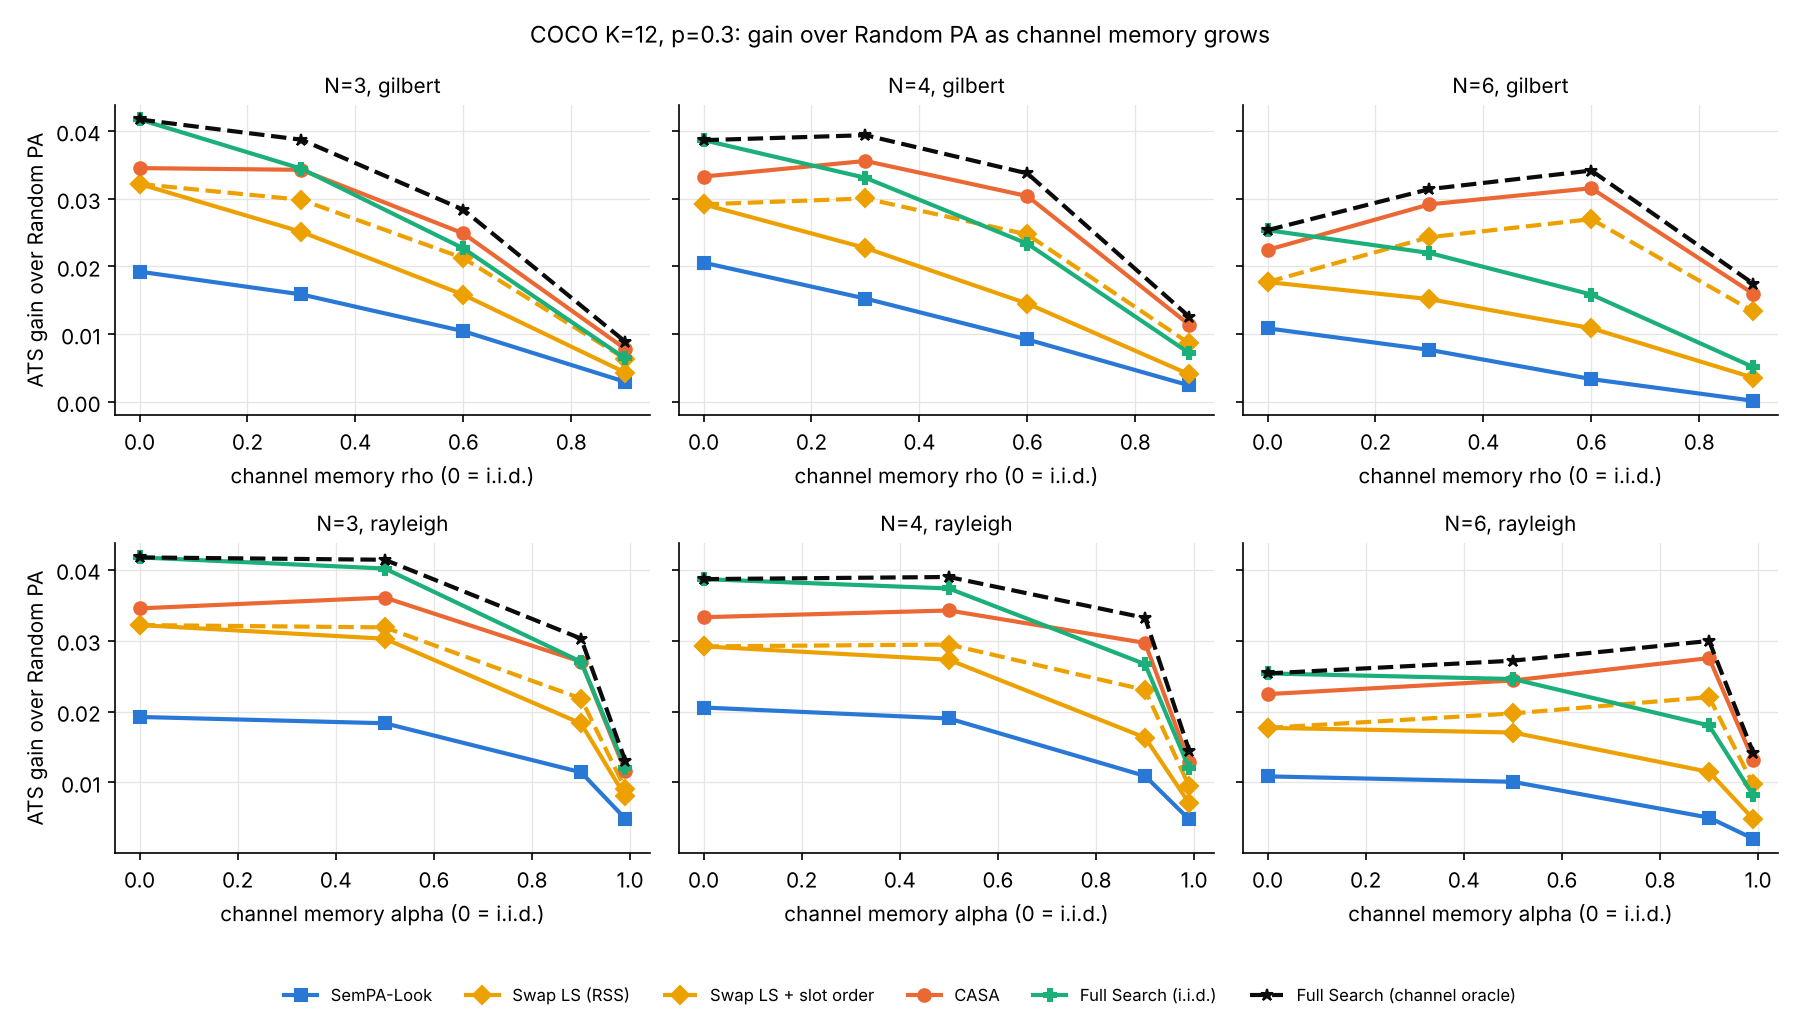
\includegraphics[width=0.62\linewidth]{coco_k12_memory_p0.3.png}
\caption{Share of the oracle's gain versus channel memory at $p=0.3$ (COCO, $K=12$). Channel-blind methods lose ground as memory grows; CASA does not.}
\label{fig:memory}
\end{figure}

\subsection{What the gain is made of}
Slot order is the cheap half: reordering SemPA-Look's own partition lifts it from 0.5998 to 0.6258 at the example point for 63 extra calls. Channel-aware grouping is the rest: CASA beats every blind method with ordering at $p\ge0.3$. Memory-blind $p$-awareness is not enough: CASA fitted as if losses were i.i.d.\ matches CASA under i.i.d.\ losses but trails it under memory (0.6177 vs 0.6387 at the example point). Seeding swap search with the interleaver changes its ATS by at most 0.002.

\subsection{Interleaving depth and delay}
A packet interleaver of depth $D$ removes much of the burst penalty for every method, at the price of a span of $(N-1)D$ packets before a message is complete. Interpolating ATS over $\log_2 D$, SemPA-Look needs a 1.5--2.3$\times$ deeper interleaver to match CASA at $D\le2$; swap search with ordering needs 1.07--1.45$\times$ at $D\le4$, rising to 1.5--1.85$\times$ at $D=8$ on the Gilbert channel with $N=6$, $p\ge0.3$. Channel-aware aggregation therefore buys roughly one doubling of interleaver depth against the paper's method, and it combines with interleaving rather than replacing it (Fig.~\ref{fig:delay}).

\begin{figure}[t]
\centering
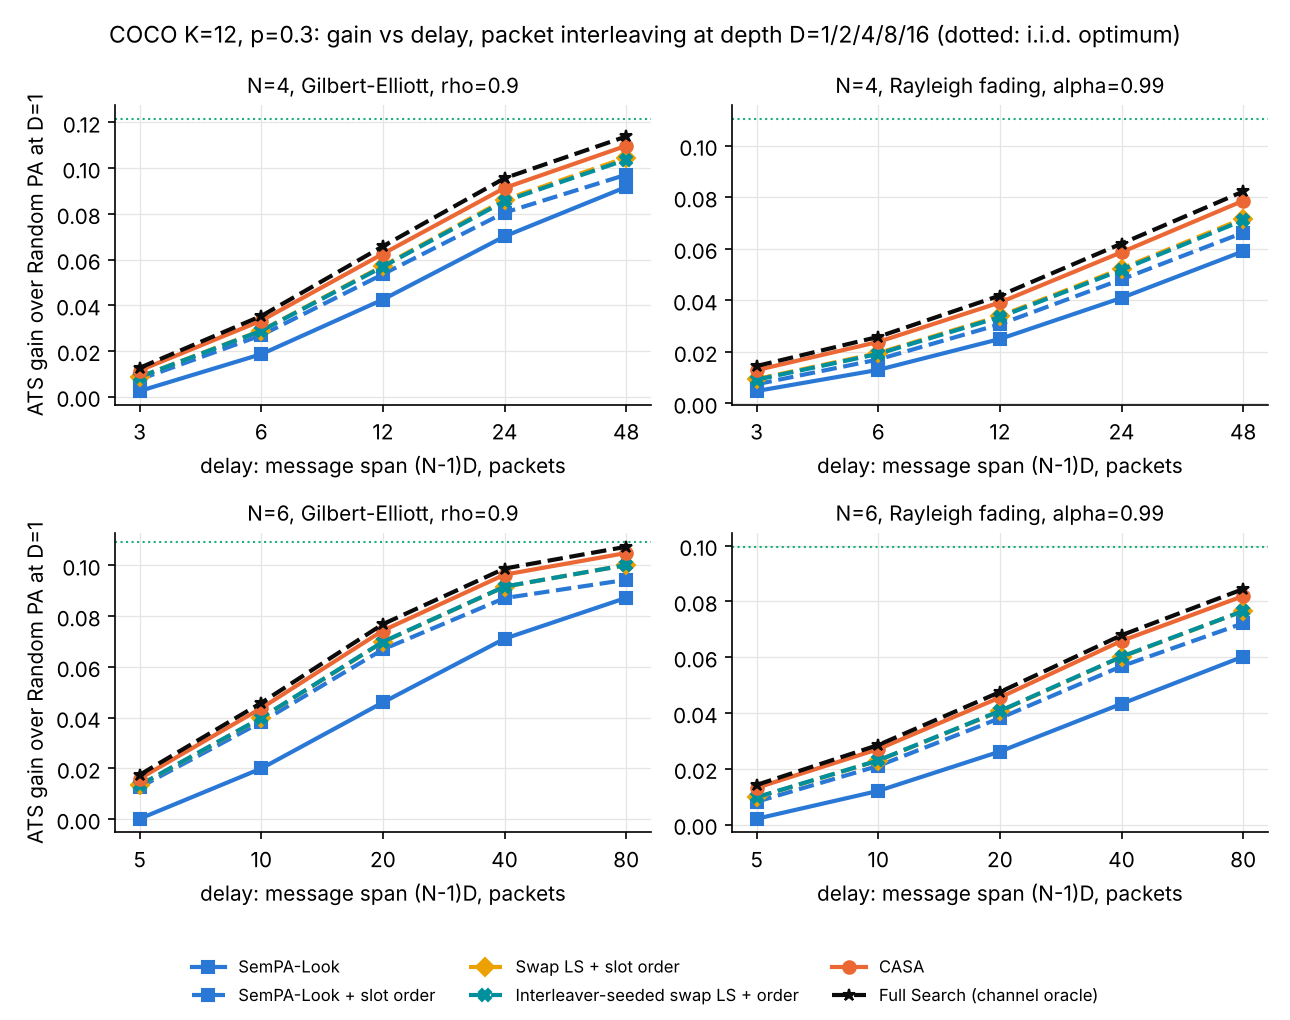
\includegraphics[width=0.75\linewidth]{coco_k12_delay_p0.3.png}
\caption{Gain over Random PA at $D=1$ versus delay span for interleaving depths $D=1,\dots,16$ (COCO, $K=12$, $p=0.3$, strong memory).}
\label{fig:delay}
\end{figure}

\subsection{Mismatched and estimated channel law}
\label{sec:mismatch}
\emph{[To be filled from \texttt{results/channel/coco\_k12\_mismatch}: CASA designed with a wrong memory parameter, a wrong family, a wrong $p$ ($\times0.5$, $\times1.5$), a Gilbert model fitted by maximum likelihood to $T\in\{100,300,10^3,10^4\}$ observed packets, and the empirical slot-pattern law from $T$ packets; scored under the true law.]}

\subsection{Metric and encoder robustness}
Partitions chosen with MPNet keep their advantage when re-scored with \texttt{all-MiniLM-L6-v2} and \texttt{bge-small-en-v1.5}: CASA's gain over SemPA-Look stays positive with CIs above zero at every bursty point, at about half (MiniLM) and a quarter to a third (BGE-small) of the MPNet size. \emph{[BERTScore F1 (RoBERTa-large, baseline-rescaled) re-score to be added.]}

\subsection{Longer messages}
Full Search is infeasible beyond $K=12$. On WikiHow $K=24$ at $p=0.5$, CASA beats SemPA-Look by $+0.056$ ATS ($+9.5\%$) on the Gilbert channel and swap search with ordering by $+0.016$. At $K=48$ and $60$ the gap to SemPA-Look grows to $+0.06$--$0.08$ at $p=0.5$, and CASA uses $2.4$--$3.3\times$ fewer encoder calls than swap search, whose cost grows with the number of token pairs. \emph{[Update with the extended samples.]}

%=====================================================================
\section{Limitations}
%=====================================================================
At low loss ($p\approx0.1$) CASA only ties a well-searched blind partition with ordering, and under i.i.d.\ losses at $K\ge48$ it trails it by 0.004. The receiver simply drops lost tokens; a generative receiver that infills missing tokens would change $\phi$ and could be modelled as another law over survival patterns. Every metric we use is automatic; none is a human judgment. If a deep interleaver is affordable, most of the burst penalty disappears for all methods, so CASA matters most under a fixed delay budget or fading too slow for the batch to average out.

%=====================================================================
\section{Conclusion}
%=====================================================================
Assuming independent packet losses hides the degree of freedom that matters most on real links: which group goes in which slot. CASA exposes it with a pairwise surrogate fitted on the channel's survival law and a closed-form quadratic assignment, and recovers most of the exhaustive oracle's gain at a few hundred encoder calls. \emph{[Final sentence on robustness to a mismatched law.]}

\bibliographystyle{IEEEtran}
\bibliography{refs}

\end{document}
